\documentclass[10pt,a4paper,oneside]{article}
\usepackage[utf8]{inputenc}
\usepackage{draftwatermark} % 设置水印
\SetWatermarkText{DNV Group} % 水印内容
\usepackage{amsmath}
\usepackage{amsfonts}
\usepackage{amssymb}
\usepackage{graphicx}
\usepackage{breqn}
\usepackage{tikz} % system block diagram
\usepackage{textcomp}
\usetikzlibrary{shapes,arrows} % system block diagram
\usepackage{booktabs}
\usepackage[framed,numbered,autolinebreaks,useliterate]{mcode} % matlab code block
\author{Yangang Cao}
\date{February 18, 2019}
\newcommand{\degree}{^\circ}
\tikzset{
	delay/.style    = {draw, thick, rectangle, minimum height = 3em,
		minimum width = 3em},
	sum/.style      = {draw, circle, node distance = 2cm}, 
	prod/.style     = {draw, circle, node distance = 2cm},
	input/.style    = {coordinate}, % Input
	output/.style  = {coordinate} % Output
}
% Defining string as labels of certain blocks.
\newcommand{\product}{$\displaystyle \times$}
\newcommand{\delay}{\large$z^{-1}$}
\begin{document}

\title{First/Second-Order Allpass Filter Design}
\maketitle 

The signal can be seen as a set of partials having different frenquencies and amplitudes. The filter can modify the amplitude of partials according to their frenquency. A special class of parametric filter structures for lowpass, highpass, bandpass and bandreject filter functions was introduced in the following articles of this series, these filter structures are easily tunable by changing only one or two coefficients. They play important roles for real-time control with minimum computational complexity.

The basis for parametric first- and second-order IIR filters is the first- and second-order allpass filter, the allpass filters don't affect the amplitude, but the phase of signal. We discuss the first- and second-order allpass filters in this text.

A first-order allpass filter is given by the transfer function
\[
A(z) = \frac{z^{-1} + c}{1 + cz^{-1}}
\]
\[
c = \frac{\tan(\pi f_c/f_S) - 1}{\tan(\pi f_c/f_S) + 1},
\]
the difference equations
\[
x(n) = u(n) - cx(n-1)
\]
\[
y(n) = cx(n) + x(n-1),
\]
and corresponding state and output equations are
\[
x(n) = -cx(n-1) +u(n)
\]
\[
y(n) = (1-c^2)x(n-1) + cu(n).
\]
which can be realized by the following block diagram.
\begin{center}
	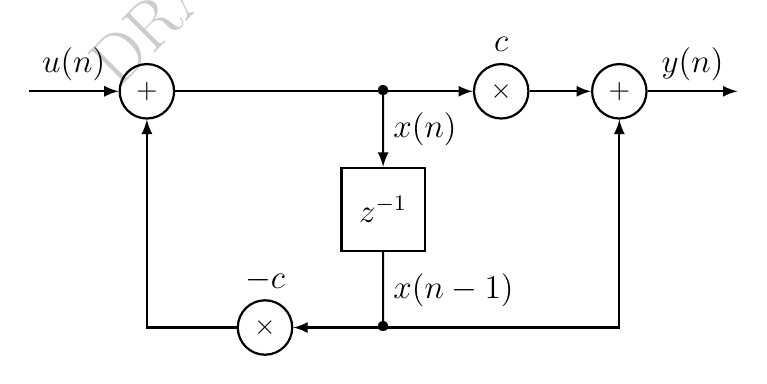
\begin{tikzpicture}[auto, thick, node distance=0.6cm, >=latex, scale = 0.75]
	\draw
	% Drawing the blocks of first filter 
	node at (0,0)[sum] (s1) {$+$}
	node at (6,0)[prod] (p1) {\product} node[above of = p1] {\large$c$}
	node at (8,0)[sum] (s2) {$+$}
	node at (4,-2) [delay] (d1) {\delay}
	node at (2,-4) [prod] (p2) {\product} node[above of = p2] {\large$-c$};
	
	\draw[->](-2,0) -- node {\large$u(n)$}(s1);
	\draw[->](s1) -- node {} (p1);
	\draw[->](p1) -- node {} (s2);
	\draw[->](s2) -- node {\large$y(n)$} (10,0);
	\draw[->](4,0) -- node {\large$x(n)$} (d1);
	\draw[->](p2) -| node {} (s1);
	\draw[-](d1) -- node {\large$x(n-1)$} (4,-4);
	\draw[<->](p2) -| node {} (s2);
	
	\draw
	node at (4,0) {\textbullet} 
	node at (4,-4){\textbullet};
	
	\end{tikzpicture}
\end{center}
A first-order allpass filter implementation can be obtained by the following {\bfseries Matlab} code.
\begin{lstlisting}
function y = firstallpassunit(audio, para)
% Applies a allpass filter to the input signal.
% para is the normalized cut-off frequency in (0,1)
c = (tan(pi*para/2)-1) / (tan(pi*para/2)+1);
x = 0;
x_1 = 0;
for n = 1:length(audio)
	x_1 = -c * x+ audio(n);
	y(n) = (1-c^2) * x + c * audio(n);
	x = x_1;
end
\end{lstlisting}

The implementation of tunable bandpass and bandreject filters can be achieved with a second-order allpass filter. The transfer function of a second-order allpass filter is given by
\[
A(z) = \frac{-c + d(1-c)z^{-1} + z^{-2}}{1 + d(1-c)z^{-1} - cz^{-2}}
\]
\[
c = \frac{\tan(\pi f_b/f_S) - 1}{\tan(\pi f_b/f_S) + 1}
\]
\[
d = -\cos(2\pi f_c/f_S),
\]
the difference equatons
\[
x(n) = u(n) - d(1-c)x(n-1) + cx(n-2)
\]
\[
y(n) = -cx(n) + d(1-c)x(n-1) + x(n-2).
\]
and corresponding state and output equations
\[
\begin{bmatrix}x(n)\\x(n-1)\end{bmatrix} = \begin{bmatrix}
-d(1-c)&c\\
1&0
\end{bmatrix}
\begin{bmatrix}x(n-1)\\x(n-2)\end{bmatrix} + \begin{bmatrix}1\\0\end{bmatrix}
u(n)\]
\[
y(n) = \begin{bmatrix}(1-c^2)d&1-c^2\end{bmatrix}
\begin{bmatrix}x(n-1)\\x(n-2)\end{bmatrix} + (-c)u(n).
\]

The parameter $d$ adjusts the center frequency and the parameter $c$ the bandwidth. The
magnitude response is again equal to one and the phase response approaches ${-360\degree}$ for high
frequencies. The cut-off frequency $f_c$ determines the point on the phase curve where the phase response passes ${-180\degree}$. The width or slope of the phase transition around the cut-off frequency is controlled by the bandwidth parameter $f_b$. The following block diagram shows the second-order allpass filter.
\begin{center}
	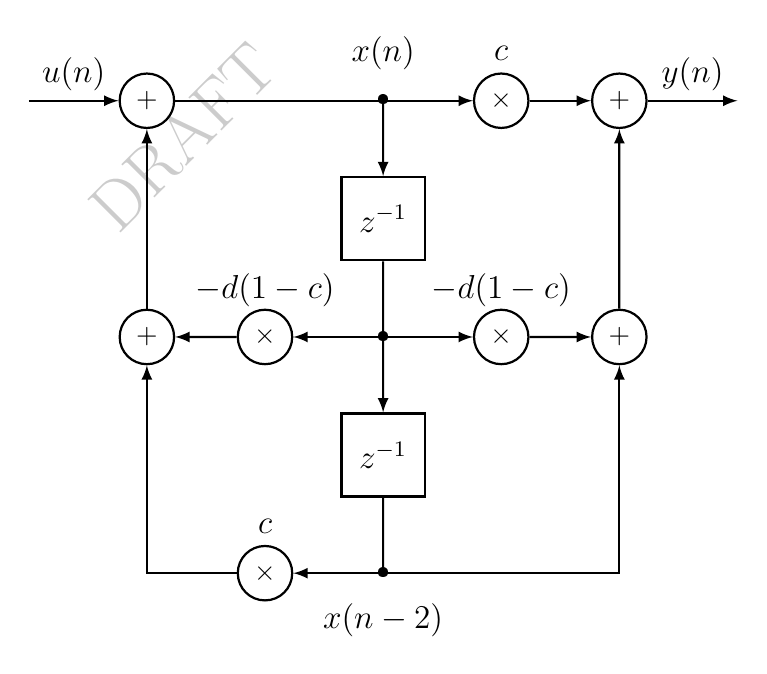
\begin{tikzpicture}[auto, thick, node distance=0.6cm, >=latex, scale = 0.75]
	\draw
	% Drawing the blocks of first filter 
	node at (0,0)[sum] (s1) {$+$}
	node at (6,0)[prod] (p1) {\product} node[above of = p1] {\large$c$}
	node at (8,0)[sum] (s2) {$+$}
	node at (4,-2) [delay] (d1) {\delay}
	node at (0,-4) [sum] (s3) {$+$}
	node at (2,-4) [prod] (p2) {\product} node[above of = p2] {\large$-d(1-c)$}
	node at (6,-4) [prod] (p3) {\product} node[above of = p3] {\large$-d(1-c)$}
	node at (8,-4) [sum] (s4) {$+$}
	node at (4,-6) [delay] (d2) {\delay}
	node at (2,-8) [prod] (p4) {\product} node[above of = p4] {\large$c$}
	 ;
	
	\draw[->](-2,0) -- node {\large$u(n)$}(s1);
	\draw[->](s1) -- node {} (p1);
	\draw[->](p1) -- node {} (s2);
	\draw[->](s2) -- node {\large$y(n)$} (10,0);
	\draw[->](4,0) -- node {} (d1);
	\draw[->](d1) -- node {} (d2);
	\draw[<->](p2) -- node {} (p3);
	\draw[->](p2) -- node {} (s3);
	\draw[->](s3) -- node {} (s1);
	\draw[->](p3) -- node {} (s4);
	\draw[->](s4) -- node {} (s2);
	\draw[-](d2) -- node {} (4,-8);
	\draw[<->](p4) -| node {} (s4);
	\draw[->](p4) -| node {} (s3);
	
	\draw
	node at (4,0)(n1) {\textbullet} node[above of = n1]{\large$x(n)$}
	node at (4,-4){\textbullet}
	node at (4,-8)(n2){\textbullet} node[below of = n2]{\large$x(n-2)$};
	\end{tikzpicture}
\end{center}
A second-order allpass filter implementation can be obtained by the following {\bfseries Matlab} code.
\begin{lstlisting}
function y = secondallpassunit(audio, para)
% Applies a allpass filter to the input signal.
% para(1) is the normalized center frequency in (0,1), i.e. 2*fc/fs.
% para(2) is the normalized bandwidth in (0,1) i.e. 2*fb/fs.
c = (tan(pi*para(2)/2)-1) / (tan(pi*para(2)/2)+1);
d = -cos(pi*para(1));
x = [0; 0];
x_1 = 0;
A = [-d*(1-c), c; 1, 0];
B = [1; 0];
C = [d*(1-c^2), 1-c^2];
D = -c;
for n=1:length(audio)
	x_1 = A * x + B * audio(n);
	y(n) = C * x + D * audio(n);
	x = x_1;
end
\end{lstlisting}
\end{document}
